\documentclass[tikz]{standalone}

\colorlet{mg}{green!50!black}
\colorlet{mb}{blue!50!black}
\colorlet{c}{cyan!70!black}

\begin{document}
\bfseries
\large 
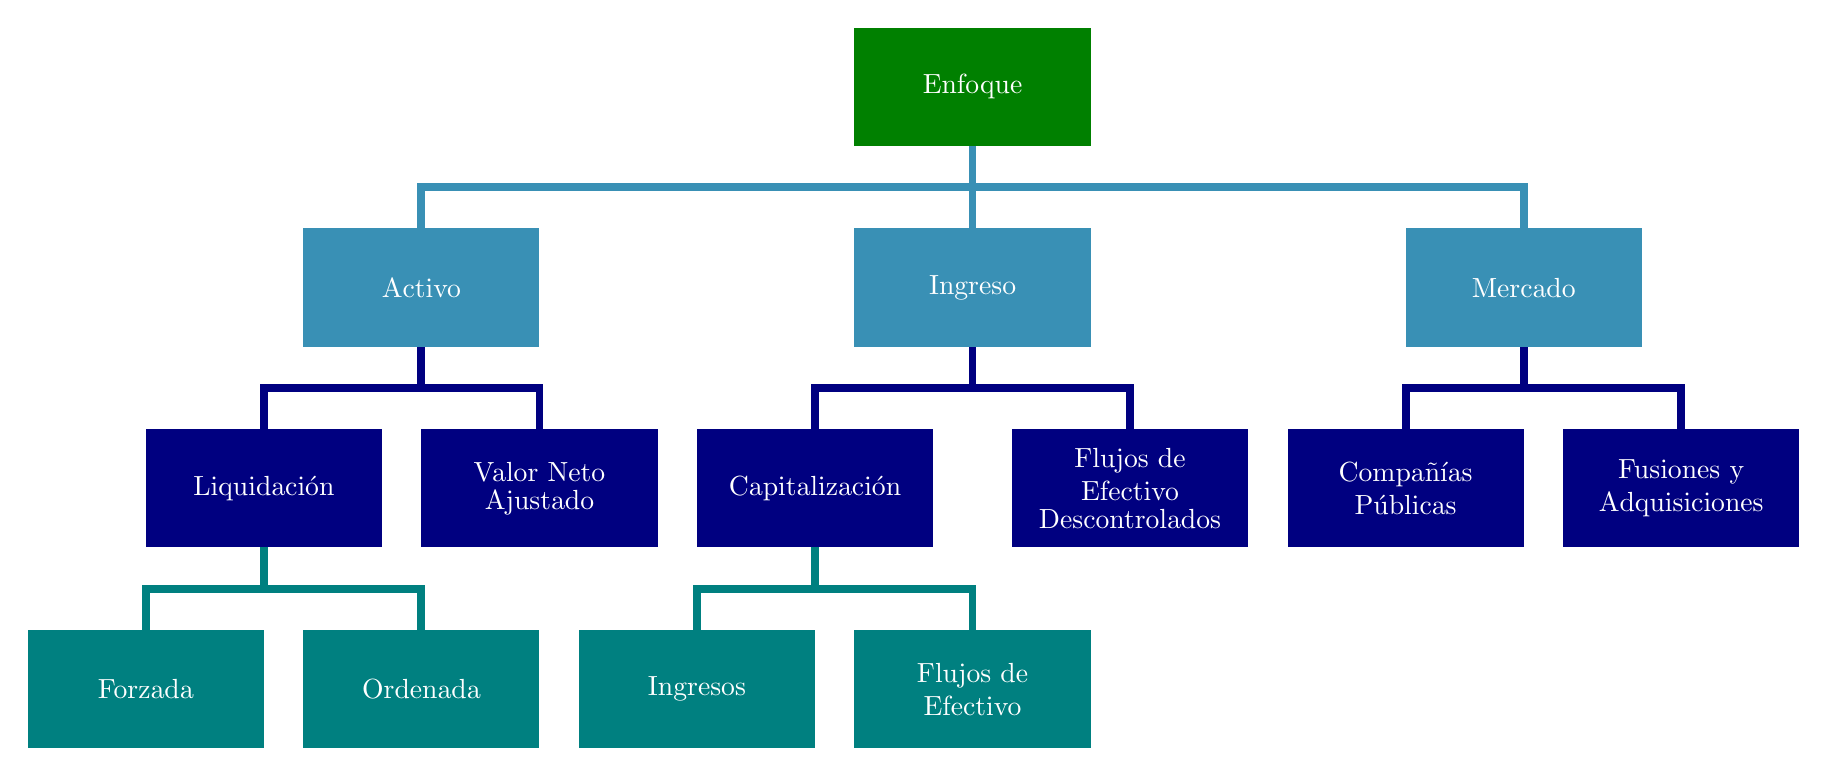
\begin{tikzpicture}[yscale=1.7,rectangle, 
	minimum height=1.5cm,
	minimum width=3cm,
	text=white]

	\coordinate (Enf)  at (0,0);
	\coordinate (Act)  at (-7,-1.5);
	\coordinate (Ing)  at (0,-1.5);
	\coordinate (Mer)  at (7,-1.5);
	\coordinate (Liq)  at (-9,-3);
	\coordinate (Val)  at (-5.5,-3);
	\coordinate (Cap)  at (-2,-3);
	\coordinate (Flu)  at (2,-3);
	\coordinate (Com)  at (5.5,-3);
	\coordinate (Fus)  at (9,-3);
	\coordinate (For)  at (-10.5,-4.5);
	\coordinate (Ord)  at (-7,-4.5);
	\coordinate (Ingr) at (-3.5,-4.5);
	\coordinate (Fluj) at (0,-4.5);

	\draw [line width=1mm,c] (Enf) -| (Ing);
	\draw [line width=1mm,c] (Enf)++(0,-0.75) -| (Act);
	\draw [line width=1mm,c] (Enf)++(0,-0.75) -| (Mer);

	\draw [line width=1mm,mb] (Act)++(0,-0.75) -| (Act);
	\draw [line width=1mm,mb] (Act)++(0,-0.75) -| (Liq);
	\draw [line width=1mm,mb] (Act)++(0,-0.75) -| (Val);

	\draw [line width=1mm,mb] (Ing)++(0,-0.75) -| (Ing);
	\draw [line width=1mm,mb] (Ing)++(0,-0.75) -| (Cap);
	\draw [line width=1mm,mb] (Ing)++(0,-0.75) -| (Flu);

	\draw [line width=1mm,mb] (Mer)++(0,-0.75) -| (Mer);
	\draw [line width=1mm,mb] (Mer)++(0,-0.75) -| (Com);
	\draw [line width=1mm,mb] (Mer)++(0,-0.75) -| (Fus);

	\draw [line width=1mm,teal] (Liq)++(0,-0.75) -| (Liq);
	\draw [line width=1mm,teal] (Liq)++(0,-0.75) -| (For);
	\draw [line width=1mm,teal] (Liq)++(0,-0.75) -| (Ord);

	\draw [line width=1mm,teal] (Cap)++(0,-0.75) -| (Cap);
	\draw [line width=1mm,teal] (Cap)++(0,-0.75) -| (Ingr);
	\draw [line width=1mm,teal] (Cap)++(0,-0.75) -| (Fluj);

	\node [fill = mg] at (Enf)  {Enfoque};
	\node [fill = c]  at (Act)  {Activo};
	\node [fill = c]  at (Ing)  {Ingreso};
	\node [fill = c]  at (Mer)  {Mercado};
	\node [fill = mb]  at (Liq)  {Liquidación};
	\node [fill = mb]  at (Val)  {\shortstack{Valor Neto \\ Ajustado}};
	\node [fill = mb]  at (Cap)  {Capitalización};
	\node [fill = mb]  at (Flu)  {\shortstack{Flujos de \\ Efectivo \\ Descontrolados}};
	\node [fill = mb]  at (Com)  {\shortstack{Compañías \\ Públicas}};
	\node [fill = mb]  at (Fus)  {\shortstack{Fusiones y \\ Adquisiciones}};
	\node [fill = teal]  at (For)  {Forzada};
	\node [fill = teal]  at (Ord)  {Ordenada};
	\node [fill = teal]  at (Ingr) {Ingresos};
	\node [fill = teal]  at (Fluj) {\shortstack{Flujos de \\ Efectivo}};
\end{tikzpicture}

\end{document}
